\documentclass[tikz,border=6pt]{standalone}
\usepackage{amsmath,amssymb}
\usetikzlibrary{arrows.meta}

% Redrawn from authentic scan: pdf_Mathematics_2022_BECE-MATHEMATICS-1990-2013_ee6bb659_p34_835.jpeg
% BECE 2011 Paper 1 Q24 — RS || WV cut by a transversal; 128 deg obtuse above WV on the
% left of the transversal; alpha acute above RS on the right of the transversal (alpha = 52 deg).
% Geometry is visually honest: the 128 deg wedge IS drawn as 128 deg, which fixes the
% transversal at 52 deg to the horizontal and makes alpha a true 52 deg acute angle.

\begin{document}
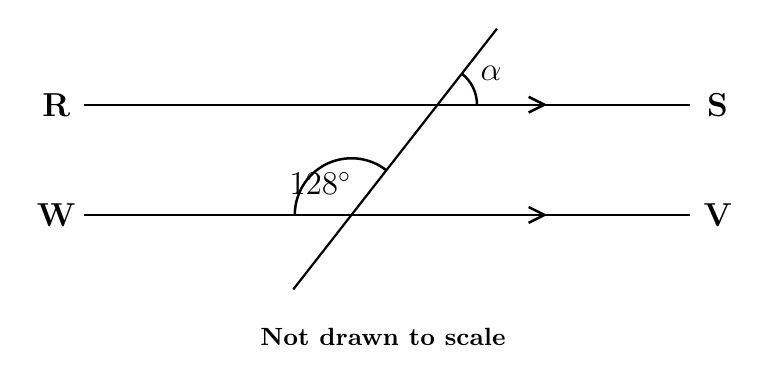
\begin{tikzpicture}[>=Stealth, line width=0.9pt]

    % ---- parallel rails ----
    \draw[thick] (-0.5, 2.6) -- (7.2, 2.6);   % top rail  R--S
    \draw[thick] (-0.5, 1.2) -- (7.2, 1.2);   % bottom rail W--V

    % ---- bold endpoint labels ----
    \node[font=\bfseries\large] at (-0.85, 2.6) {R};
    \node[font=\bfseries\large] at ( 7.55, 2.6) {S};
    \node[font=\bfseries\large] at (-0.85, 1.2) {W};
    \node[font=\bfseries\large] at ( 7.55, 1.2) {V};

    % ---- parallel marks (chevrons) on both rails ----
    \draw (5.15, 2.5)  -- (5.35, 2.6)  -- (5.15, 2.7);
    \draw (5.15, 1.1)  -- (5.35, 1.2)  -- (5.15, 1.3);

    % ---- transversal: the 128 deg wedge fixes its direction at 52 deg ----
    % lower intersection P2 = (2.9, 1.2); upper intersection P1 = (3.994, 2.6)
    \draw[thick] (2.161, 0.254) -- (4.747, 3.564);

    % ---- alpha arc: above RS, right of the transversal (0 deg .. 52 deg) ----
    \draw (3.994, 2.6) +(0.50, 0) arc[start angle=0, end angle=52, radius=0.50];
    \node at (4.672, 2.997) {\large$\alpha$};

    % ---- 128 deg arc: above WV, left of the transversal (52 deg .. 180 deg) ----
    \draw (2.9, 1.2) +(52:0.72) arc[start angle=52, end angle=180, radius=0.72];
    \node at (2.504, 1.604) {\large$128^\circ$};

    % ---- authentic BECE caption ----
    \node[font=\bfseries\small] at (3.3, -0.35) {Not drawn to scale};

\end{tikzpicture}
\end{document}
